\chapter{引言}\label{chap:introduction}

\section{研究背景与意义}

% 问题 -> 
% - 数据中心规模不断扩大
% - 提升利用率的重要性
% 解决方式 -> 混部技术
% - LS 和 BE 应用天然具备混部
% - 通过混部的确解决了问题
% 局限 -> QOS
% 本质 -> 混部共享资源的竞争
% - CPU\Cache\Memory\IO\Net
% - AVX
% 研究现状
% - 劣化监测
% - 调度
% 本文

云计算为用户提供了使用计算资源的便捷方式,虚拟化技术让云计算服务具备了弹性、安全等特征,大大减轻了云用户的管理负担。随着LXD、Docker等容器技术发展,轻量的隔离技术让应用能更方便地进行分发与管理,大大降低了应用上云的难度,同时,随着K8s、OpenShift等容器编排技术发展,DevOps概念逐渐成熟并广泛实践,创造了更便捷、灵活的开发运维模式,这些都使得企业与普通用户倾向于在云平台上部署应用。而不断扩张的需求催生了巨大的云计算市场,为满足庞大的市场需求,云厂商不断地扩大数据中心规模,据中国信息通信研究院中国算力发展指数白皮书(2023年)显示,2022年国内数据中心机架规模超过650万个标准机架,基础算力规模达到180EFlops,位居全球第二\citep{chinaict2023}。

数据中心的庞大规模带来了巨大的治理挑战。头部云厂商微软Azure在其内部调研中发现,数据中心每减少1\%的资源分配碎片率,每年就能节省近1亿美元\citep{hadary2020protean}。在数据中心规模不断扩张的背景下,高效利用数据中心计算资源、提高整体资源利用率是云厂商关注的核心问题。

通过将互补类型的应用部署到相同物理机上,实现数据中心利用率的提高是数据中心混部技术的主要方式。数据中心通常依据应用对延迟的敏感度,将应用划分为延迟敏感性(LC)与尽力交付型(BE)两类。其中,延迟敏感性应用通常为交互型应用,如在线购物等,这类应用对延时十分敏感,需要保持运行。尽力交付型应用通常为离线应用,如大数据处理等,这类应用对延迟几乎没有要求,允许中断和重新运行。LC应用负载具有明显潮汐特征,而在LC应用的各个空闲时段填充BE应用是混部能够提升资源利用率的关键。实践中,阿里云通过混部技术分别将集群的平均CPU利用率和内存资源利用率提升到了38.2\%和88.2\%\citep{guo2019limits}。

\begin{figure}[!htbp]
    \centering
    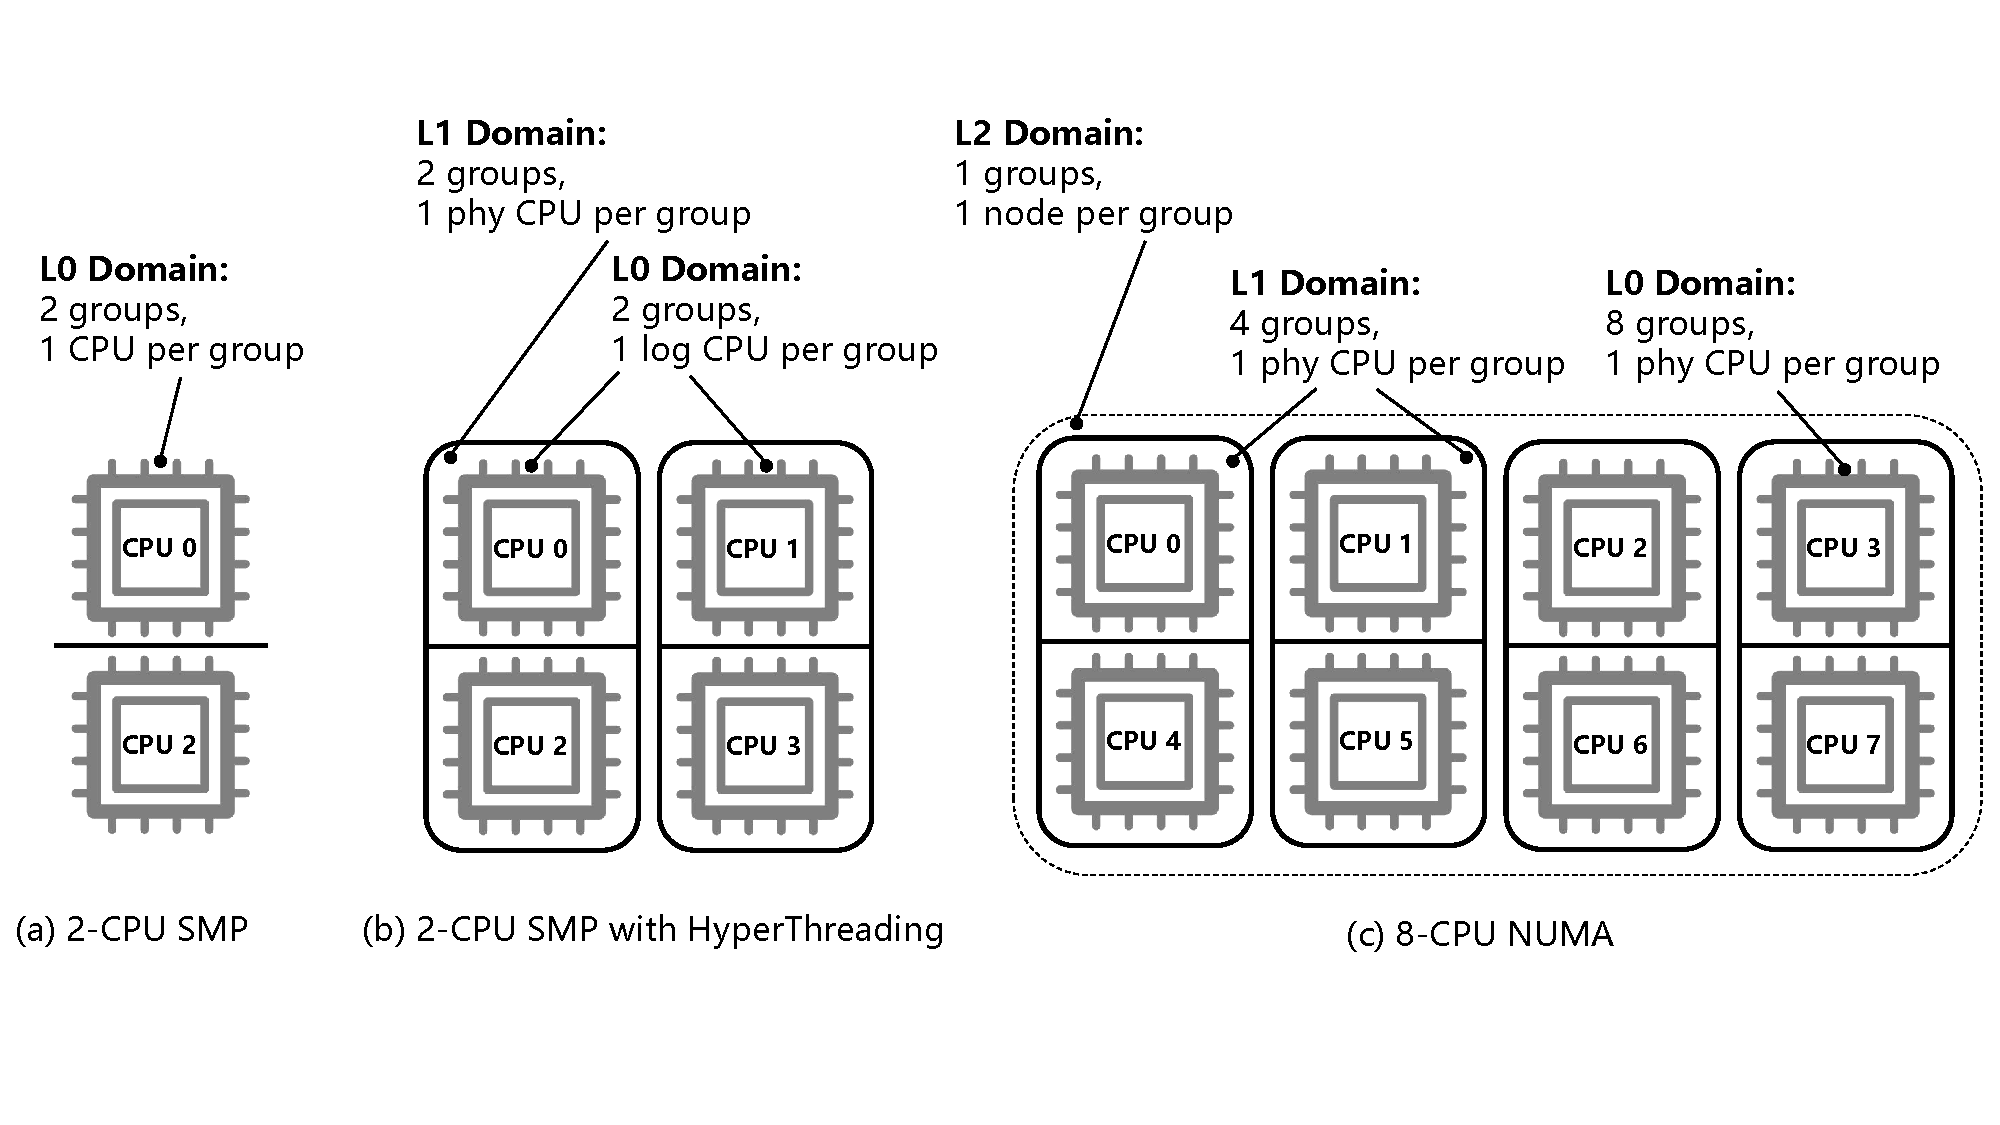
\includegraphics[width=0.85\textwidth]{scheduling_domain}
    \bicaption{\quad CPU拓扑}{\quad CPU Topology}
    \label{fig:scheduling_domain}
\end{figure}

资源竞争是混部场景中不可忽略的主要问题。现代服务器计算资源丰富,能够支持大量应用同时运行。然而服务器的局部硬件处理能力有限,如片上资源、LLC、内存带宽、网络等。混部试图向单一服务器上引入更多任务,这无疑增大了局部硬件资源竞争的概率。如在网络子系统中,任务在内核处理关键路径上的积压,会引发整体延迟的上升。同时,数据中心应用数量多、软件环境复杂,不同应用对于服务器资源的需求各不相同。这就导致一方面,数据中心应用之间存在许多隐含的资源竞争,另一方面,资源竞争引发的应用性能劣化程度也有所不同。

资源竞争的核心是资源的共享性与有限性。CPU是重要的共享资源,随CPU设计与制造技术的不断进步,服务器上CPU资源拓扑也越来越复杂。当前如超线程技术(Hyperthreading)、非同一内存访问架构(NUMA)、大小核心架构等CPU架构上的新特性给Linux调度巨大的挑战。如图~\ref{fig:scheduling_domain}所示,逻辑核通常是最底层的拓扑,在同一个逻辑核心上任务分时复用CPU资源,某一时刻仅有一个任务在运行,彼此几乎不存在影响。超线程由Intel公司最早于2002年引入市场,使得一个物理核心上能够存在多个逻辑核心。如图~\ref{fig:cpu_topology}所示,超线程兄弟核心拥有独立的寄存器组与中断控制器,但彼此共享了执行单元、Cache和总线等其他资源。NUMA(非一致存储器访问)架构中允许有多个CPU模块,每个CPU模块可以包含多个CPU,这些CPU拥有自己的本地内存与IO接口,但彼此共享了相同的内存总线与LLC,并且在IO资源上也会相互竞争。

\begin{figure}[!htbp]
    \centering
    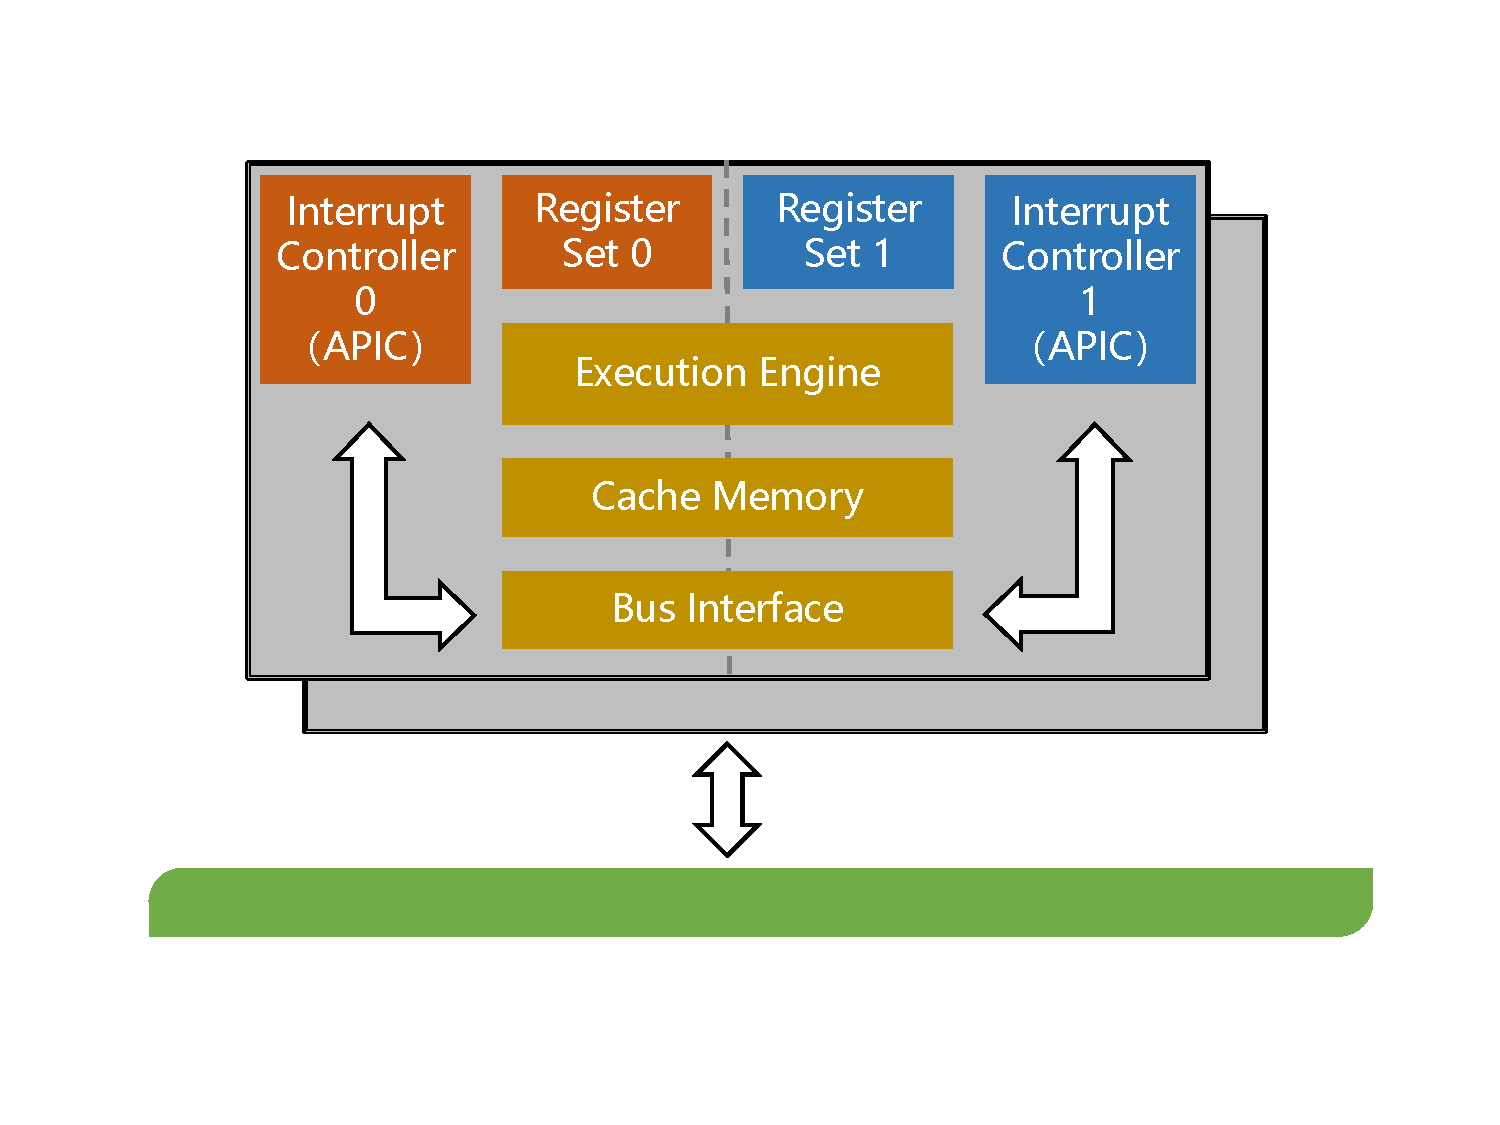
\includegraphics[width=0.6\textwidth]{cpu_topology}
    \bicaption{\quad Siblings片上共享资源 }{\quad Siblings on-chip shared resources}
    \label{fig:cpu_topology}
\end{figure}

资源竞争所导致的QoS劣化体现在应用的性能指标上,云厂商提供了SLO(Service-level objective)服务级别目标来允许用户指定云应用的期望状态。SLO中通常包含服务可用性、带宽等基础指标,也包括每秒请求数量、尾延迟等业务性能指标。云厂商通过与用户协商SLO来定义云产品的质量保证,并在违反SLO时进行补偿。

高优先级应用的QoS劣化会为云厂商带来较大损失,一方面是SLO破坏所产生经济损失,另一方面是用户流失。保障应用QoS是混部场景下云厂商核心需求,而了解应用的状态变化,实施精准的调度是解决混部场景中QoS保障问题的核心。当前混部场景下QoS保障相关研究通常从三个方向展开:

\begin{enumerate}
    \item 利用可观测性技术来对应用进行劣化监测,同时收集数据以进行画像分析。首先,云厂商依赖可观测性基础设施,来对数据中心进行持续监测,可观测性基础设施围绕不同的软件环境设计,如面向虚拟机、面向容器编排系统等,通过对目标进行全面地观测,一方面,利用实时收集的数据及时发现应用性能的劣化来进行预警,另一方面,利用丰富的指标数据来进行细致地画像分析,从而挖掘出更多的混部机会,2011年,Google公开了其数据中心混部集群监控数据集,阿里云也在2017年公开了一部分混部集群的监控数据集\citep{guo2019limits},这些来自实际生产环境的脱敏数据集,极大促进了混部策略的相关研究。
    \item 围绕资源隔离的混部场景QoS保障研究。资源隔离即通过软硬件手段来强化混部场景下应用在共享资源上的隔离性,防止因敏感资源的竞争导致应用QoS劣化。不同资源隔离技术的区别在隔离资源的类型与粒度上,使用Cgroup技术能够对CPU资源进行划分,而使用traffic control技术\citep{hubert2002linux}则能够在网络资源上进行隔离,同时,基于硬件的隔离技术粒度则更细,如Intel RDT技术\citep{guide2011intel}能够隔离末级缓存与内存带宽。通过组合这些隔离技术,来制定不同的调度策略是基于资源隔离混部研究的主要方式。
    \item 围绕任务调度的混部场景QoS保障研究。任务调度是通过修改CPU资源分配的逻辑,来间接地控制应用之间的资源竞争。任务只有被分配到CPU资源时才能执行,并获取后续的其他硬件资源,因此CPU资源是大部分硬件资源的分配起点。相关研究从任务调度的速度与灵活性上展开,其中微秒级调度机制通过实现远低于任务延迟要求的调度延迟,及时地分配CPU资源来避免QoS劣化。灵活的任务调度策略能够便于针对混部场景的不同应用与硬件特性进行针对性的定制,从而更好地满足混部场景的需求与QoS保障目标。
\end{enumerate}

\section{国内外相关研究}

\subsection{数据中心可观测性与劣化监测研究现状}

% 可观测性系统
% - 定义
% - 实践

可观测性技术指通过指标监控、日志记录、链路追踪和其他数据收集手段来描述系统的状态,从而协助理解和诊断系统的行为和性能。在指标监控上,开源社区Prometheus\citep{brazil2018prometheus}提供了标准采集数据编解码格式以及一套基本的采集系统组件。在各个厂商及开发者的共同参与下,Prometheus社区发展迅速,并逐渐成为指标采集领域的现行标准,被各个云厂商采用。

随软件架构的不断迭代,可观测性技术也在进步。微服务是数据中心常见的软件架构,一次请求调用链路往往跨越多个进程与服务器。传统的进程观测手段难以有效地对微服务进行观测,为解决这一问题,2010年Google提出了分布式链路追踪系统Dapper\citep{sigelman2010dapper}。Dapper用于对微服务应用进行性能分析,其中,使用Trace来记录一次完整的链路追踪,而使用Span来记录对于链路中单个操作。单个操作可以是一次函数的调用,也可以是一个代码块,Dapper需要用户在要追踪的位置进行代码插桩以指示Span信息的生成。在函数调用的过程中,Span会作为上下文的一部分传递给子过程,从而建立Span之间的父子关系。而在微服务中,一次函数调用也可以是一次远程过程调用(RPC),Dapper会将Span注入到请求报文的载荷中,使得Span能够跨进程、服务器地传递。所有的Span最终都会发送到Dapper的分析系统中,并根据相互之间的树形关系重建为完整的Trace过程,实现一次链路追踪。OpenTracing和OpenTelemetry等开源项目吸收了Dapper的核心思想,并迅速在云原生社区中推广。此外,CNI(Container Network Interface)\citep{k8s-network-plugins}技术允许开发者自定义容器网络模型,Cilium\citep{cilium}基于eBPF、Envoy等技术\citep{ebpf,envoyproxy}构造Overlay Network,从而实现无侵入的网络性能监测与控制。近年来随DevOps技术的发展,可观测性技术在云服务中占据了越来越重要的地位。

\begin{figure}[H]
    \centering
    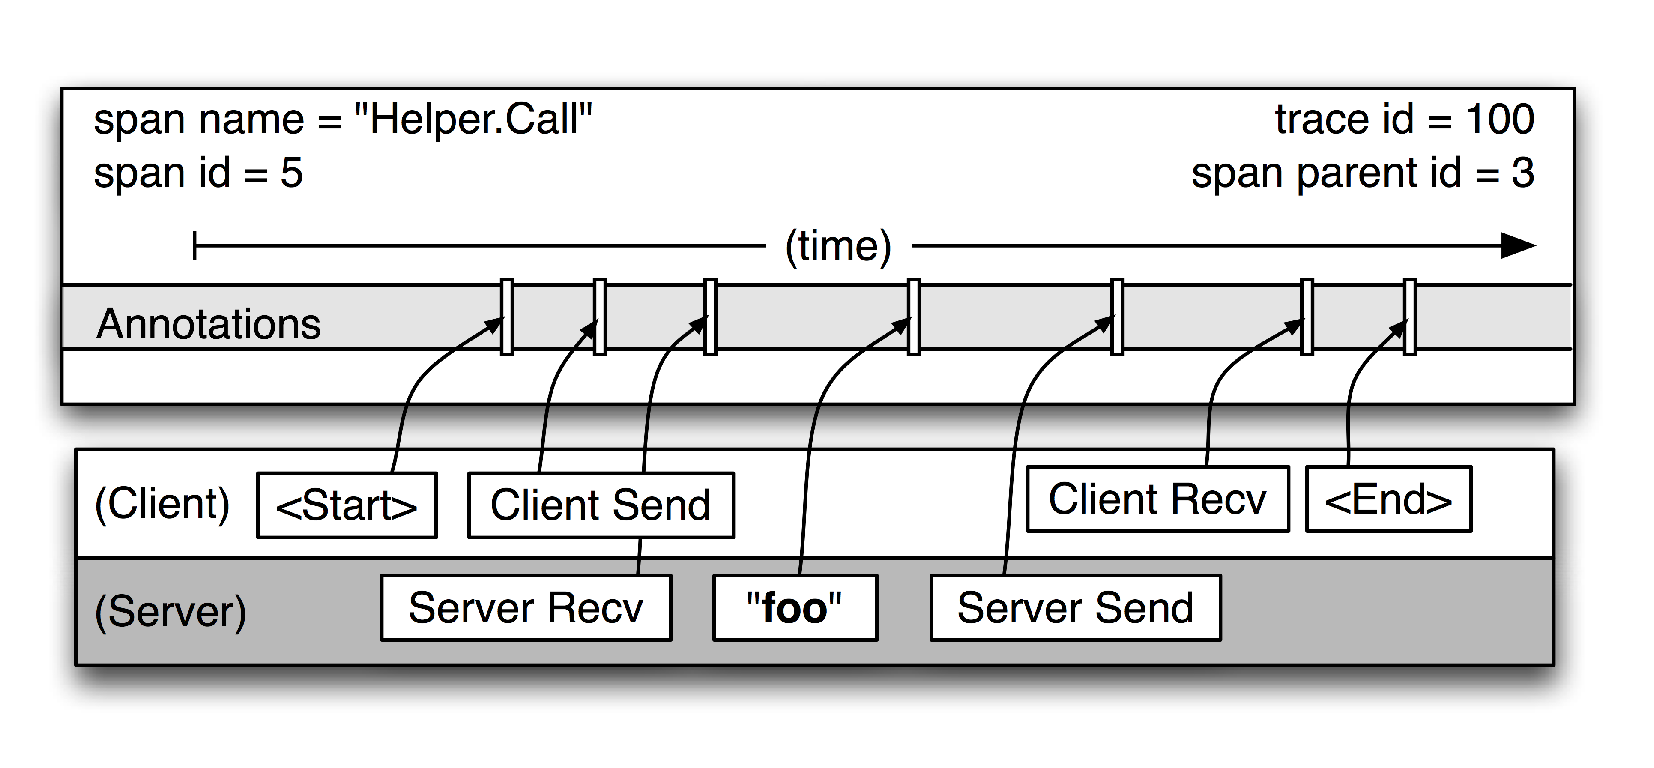
\includegraphics[width=0.6\textwidth]{dapper_span}
    \bicaption{\quad Dapper链路追踪流程(图片引用自文献\citep{sigelman2010dapper})}{\quad Dapper tracking process (picture quoted from paper\citep{sigelman2010dapper})}
    \label{fig:parties_app_dif}
\end{figure}

基于采集得到的指标来分析应用的性能劣化情况是可观测系统的主要功能之一,数据中心中由于应用数量众多、软件环境复杂,早期云厂商倾向于一些简单易懂的指标,来反映应用的性能,如Google就使用CPI\citep{zhang2013cpi2}来作为应用的性能指标。CPI(Cycle Per Instruction)本身用于度量微观体系结构下的性能,应用正常运行时,CPI通常在一个小范围内波动,而当应用受到干扰导致性能下降时,通常就能在CPI指标上体现。后续在Li YI等人的研究中\citep{yi2020cpi}发现CPI在核心频率较低时存在较大的误差,并利用建模分析优化得到RCPI来对误差进行修正。随AI技术的不断发展,研究者们发现数据中心的监控数据作为时序数据能够很方便地利用现有的AI数据分析技术进行分析,将AI和系统结合的研究也不断展开,而通过时序数据对服务性能劣化进行预测\citep{qiu2020firm, zhou2022aquatope, wang2022deepscaling, gan2021sage, ghafouri2020survey,zheng2020web,wu2019posterior},也使得提前一步进行QoS保障成为可能。FIRM\citep{qiu2020firm}面向K8s集群设计了一种两级的机器学习模型来识别集群中服务性能劣化,并在实验中取得了相当显著劣化监测与调度效果。而同时Di Wu\citep{wu2020data}则提出了一种数据特性感知潜在因素(DCALF)模型来实现高精度的QoS预测,能够依据不同QoS数据的特性来分别的进行预测。

\subsection{围绕资源隔离的混部场景QoS保障研究现状}

% 集群维度: 放置策略
% 单点维度: 细粒度分配

数据中心的资源通常可划分为集群资源与节点资源。其中,围绕集群资源隔离的研究通常可转化为任务放置问题。首先,集群的各个节点都部署有可观测性基础设施,获取集群各个节点的总体资源、资源使用情况等信息。随后,有新任务提交并需要调度到某一个节点上时,调度器就需要综合各个节点的资源信息以及任务的资源需求求解出最优的节点。Protean\citep{hadary2020protean}是微软Azure实现的面向虚拟机混部的调度系统,通过在地域、地区、机柜等各个层次上逐层决策求解出最优节点,保证给虚拟机分配所需的资源,从而避免因资源不足导致的QoS劣化。

而在节点资源上,相关研究通过软硬件手段隔离不同应用的资源,避免关键资源上的竞争来实现应用的QoS保障。节点上有丰富的资源隔离机制,在软件上,Linux内核提供了丰富的资源隔离机制,如Cgroup、traffic control。在硬件上,为解决"吵闹邻居"问题\citep{xu2018dcat, maricq2018taming, rzadca2020autopilot, kwon2020dc},硬件厂商也提供更细粒度的硬件隔离机制,如Intel RDT、ADM PQoS\citep{amdpqos}、ARM MPAM\citep{armmpam}等。

基于上述的软硬件资源隔离手段,Paragon\citep{delimitrou2013paragon}、Quasar\citep{delimitrou2014quasar}预先对应用进行观测,并基于观测数据建立分类模型,当应用调度时,结合观测数据与分类模型确认应用的类型,来利用类型信息来辅助进行后续的资源隔离决策。Heracles\citep{lo2015heracles}从应用资源敏感度的角度着手,分析不同应用在不同负载下对于多种资源的敏感度,调度时依据分析结果优先保证应用的敏感资源供给,从而实现应用的QoS保障。Parties\citep{chen2019parties}分析了更多种类应用的资源敏感度,如图~\ref{fig:parties_app_dif}所示。Parties在调度上不同于Heracles,在保障QoS的前提下通过在应用之间拆借资源来提升整体资源利用率。CLITE\citep{patel2020clite}利用贝叶斯优化构建资源隔离模型,将多个LC应用与BE应用进行混部,并利用Intel MBA来对内存带宽进行控制,从而保障LC应用的QoS需求。LIBRA\citep{zhang2021libra}则基于一种新型硬件节流机制,实现内存带宽的动态调控,并根据应用的需求变化动态调整,及时地保障内存带宽资源供给。

\begin{figure}[!htbp]
    \centering
    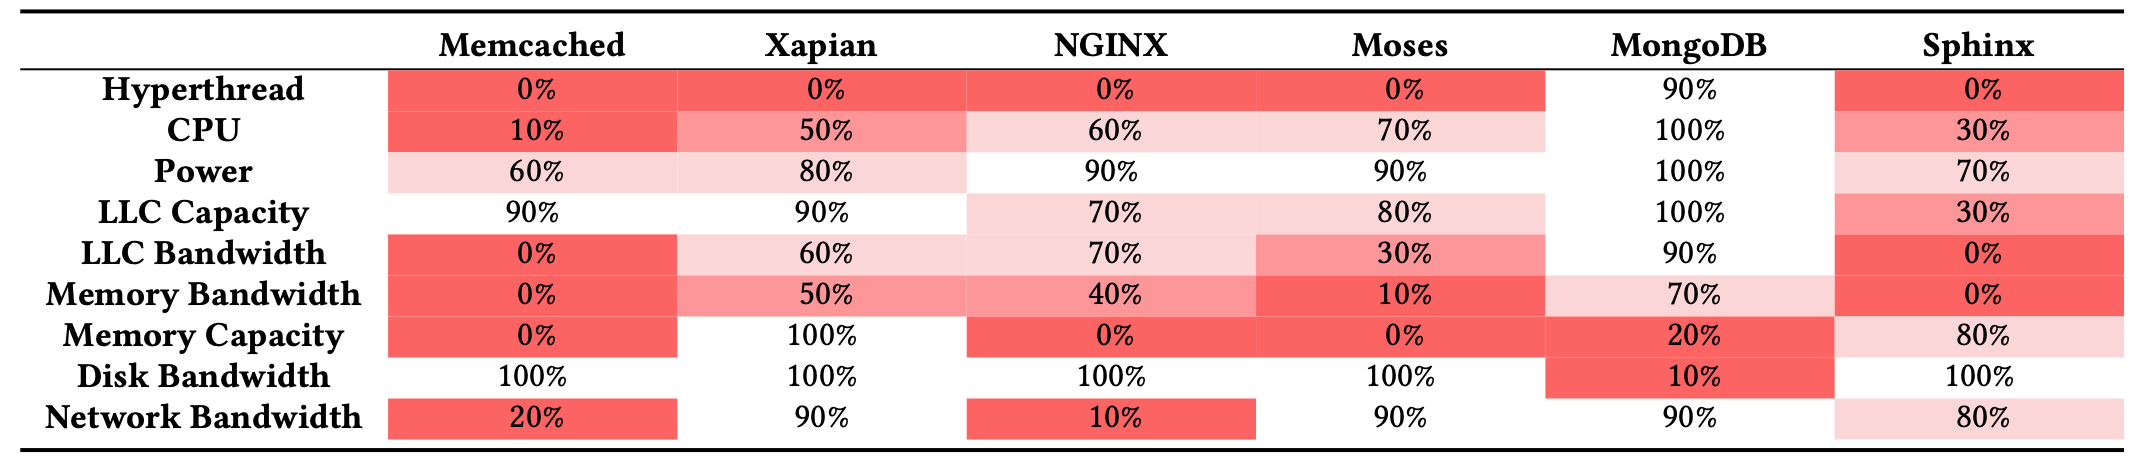
\includegraphics[width=1.0\textwidth]{parties_app_dif}
    \bicaption{\quad 不同资源干扰对应用性能的影响(图片引用自文献\citep{chen2019parties})}{\quad Impact of diferent resource interference on application performance (picture quoted from paper\citep{chen2019parties})}
    \label{fig:parties_app_dif}
\end{figure}

\subsection{围绕任务调度的混部场景QoS保障研究}

% 内核任务调度
% 微秒级调度

围绕任务调度的QoS保障研究聚焦于CPU资源分配上,相关研究通常围绕调度机制的设计展开。调度机制的核心在于调度延时与调度策略,其中调度延时通常与Runtime的实现相关,而调度策略则取决于不同混部场景的调度目标。

Linux内核任务调度中较典型的是Fair调度类,其中CFS调度器\citep{pabla2009completely}是Linux中的默认调度器,最早于2009年提出,设计目标是解决交互式应用与非交互式应用调度的公平性问题。CFS的核心在于CPU vruntime的计算与维护,对于Run Queue中的每一个调度实体,CFS会维护一个时间记账信息,并在每个时钟中断根据不同调度实体的优先级更新记账信息,优先级越高的调度实体,vruntime的积累速度越慢。随后,在每个调度循环中,CFS会选择Run Queue中vruntime最小的调度实体中的进程运行。CFS中使用了许多启发式的策略,在大多数场景下都能公平地进行调度,然而在混部场景中,部分启发式逻辑会导致严重的QoS劣化问题。如CFS调度器会为每个调度队列维护一个基准vruntime值,并将其赋予新创建的或新唤醒的进程。基准vruntime通常为Run Queue中的最小值,以便于新创建或新唤醒的进程优先执行。在LC与BE混部的场景中,为保障LC应用资源的优先供给,通常会提高LC应用的优先级,使得在每个调度循环中LC应用都有更大的几率被选中执行。然而此时如果有新创建的或新唤醒的进程,在CFS的启发式策略下这些进程会抢占高优先级的LC应用。当新创建或新唤醒的进程数量较多时,LC应用容易因得不到及时的调度而引发严重的QoS劣化。

为解决CFS存在的种种问题,2023年Linux 6.6版本中引入了EEVDF来替换CFS。EEVDF算法\citep{stoica1995earliest}提出于1995年,首先,调度器会为每个进程维护一个虚拟截止时间,并在每次调度时选择最早截止时间的任务执行,而不同于CFS,EEVDF的优先级设计考虑到了应用对延迟的不同需求,并引入了latency-nice机制,如图~\ref{fig:eevdf_scheduling}所示,为任务设置较高的latency-nice值,会让此任务总是获得长而少的时间片,对于计算密集型的应用而言,这样能够减少上下文切换的次数,从而有利于总体吞吐,而为应用设置较低latency-nice值,会让任务总是获得短而多的时间片,这样能够让CPU资源更快地分配,同时其也更容易被调度。

\begin{figure}[!htbp]
    \centering
    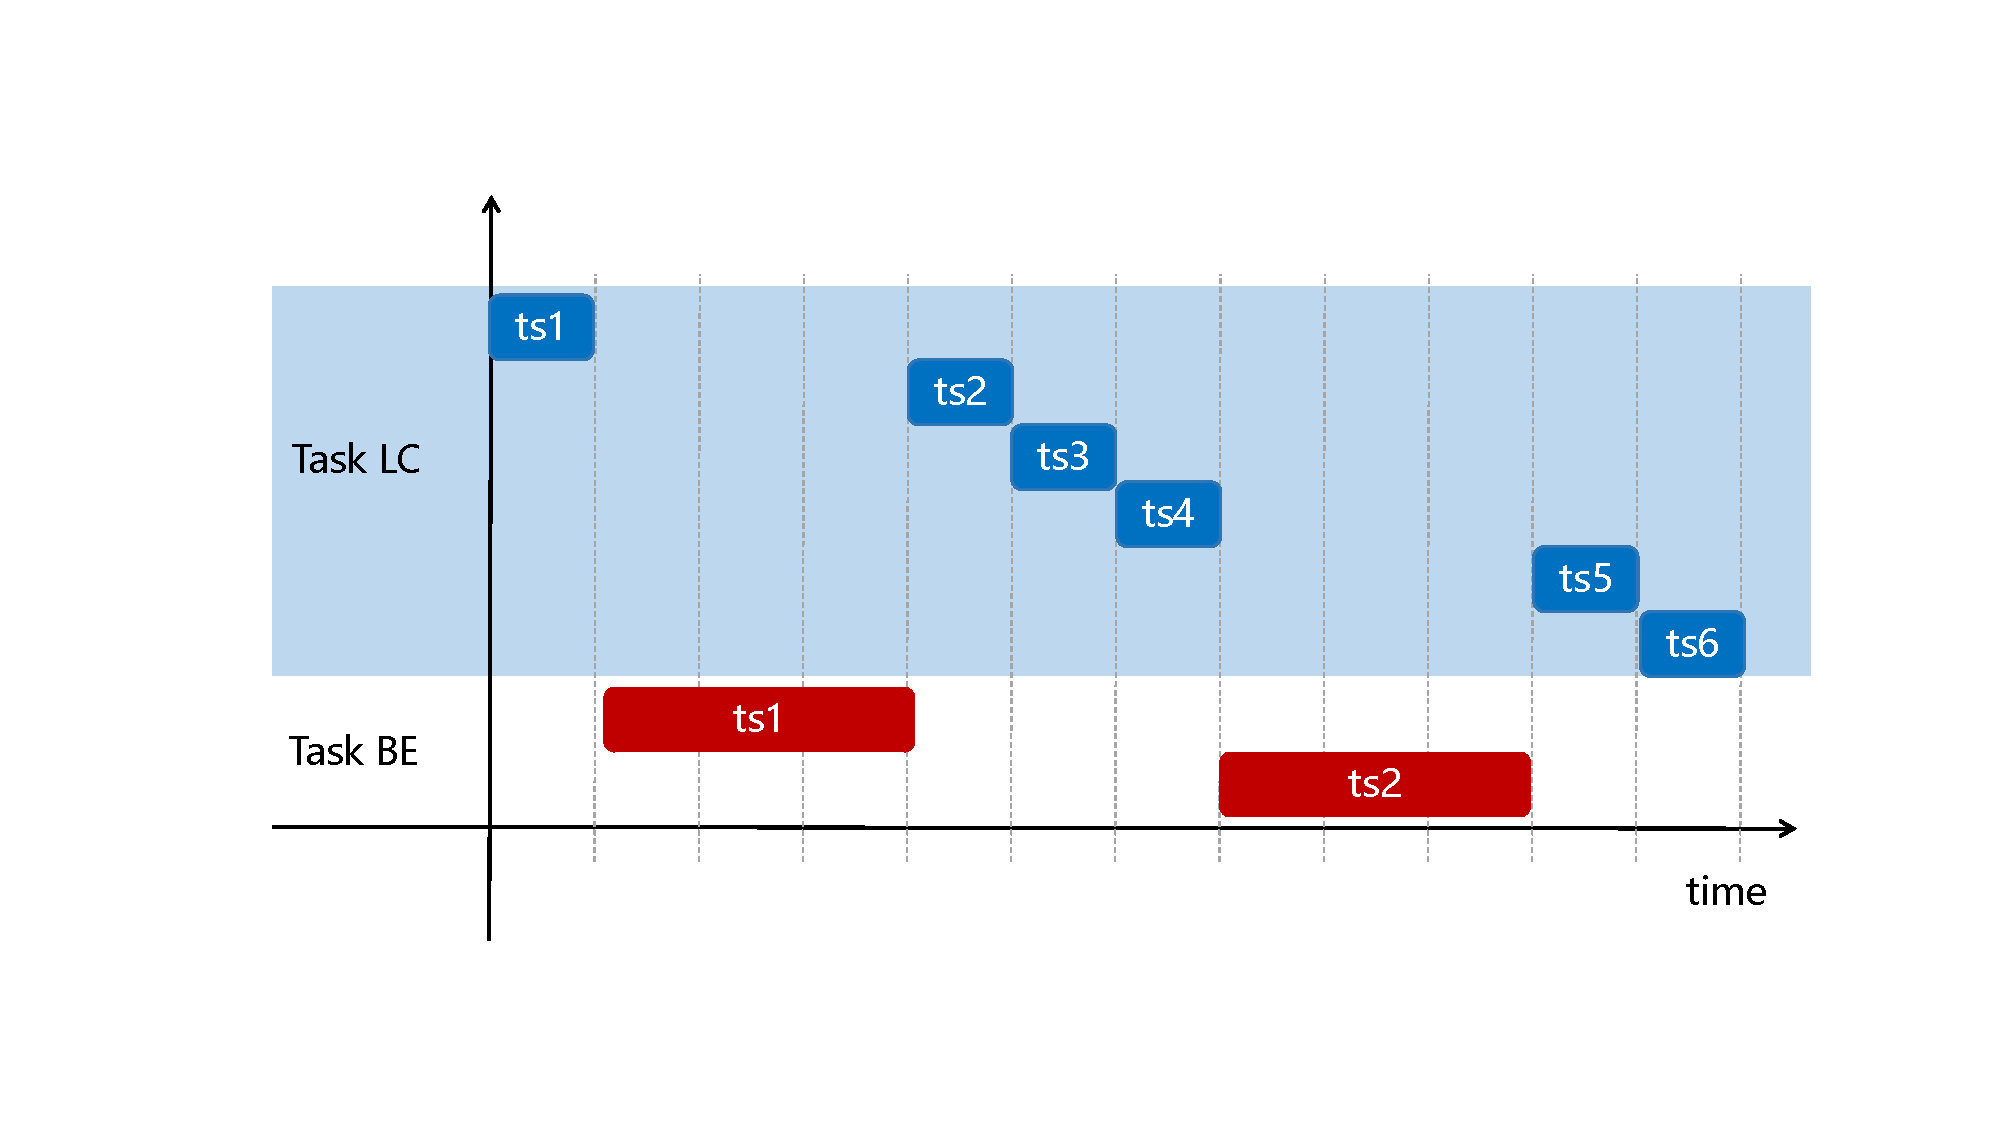
\includegraphics[width=0.8\textwidth]{eevdf_scheduling}
    \bicaption{\quad EEVDF可变时间片机制}{\quad EEVDF Variable Time Slice Mechanism}
    \label{fig:eevdf_scheduling}
\end{figure}

Linux 2.6中首次引入了调度域(Scheduler Domains)\citep{schedulerdomains},用来协助处理多核处理器上的调度,如表~\ref{tab:resourcesharing}所示,调度域充分反映了围绕CPU的共享资源信息,而通过提供这一层抽象,能够让调度子系统感知CPU之间的拓扑关系,进而做出针对性的调度决策,然而,Linux任务调度机制在适应不同调度域上仍然存在不足。超线程技术下的兄弟核心存在共享的片上资源,任务在兄弟核心上的竞争会引发性能的劣化,为解决在超线程硬件上的混部QoS保障问题,Elfen\citep{yang2016elfen}设计了一种新的内核调度机制,并提供nanonap系统调用,允许进程快速地暂时释放CPU资源,混部场景中BE应用通过代码插桩,在微秒级粒度执行兄弟核探测代码,一旦发现兄弟核上有任务允许,就立即通过nanonap系统调用释放CPU资源。其次,Linux任务调度机制在处理AVX指令时也存在问题,AVX指令(高级向量扩展)\citep{guide2011intel} 最初由Intel提出,并于2011开始在实际产品中加入。AVX指令是SIMD的一部分,旨在提高CPU的浮点运算性能。AVX指令涉及到CPU中加速单元的使用,通常使用加速单元意味着更高的能耗,CPU设计时为了防止芯片过热,会在加速单元工作时降低物理核心的运行频率。AVX指令引发了调度的两个公平性问题,首先,当降频发生在任务切换时,由于频率的恢复需要一定的时间,这使得同一逻辑核上的先后两个任务存在相互相影响的可能,其次,超线程的兄弟核心共享了同一个物理核,物理核心的降频会使得所有兄弟核心受到影响,Linux任务调度机制并没有对如上两种情况进行特殊处理,因此存在调度公平性的隐患,为解决这一问题Gottschlag\citep{gottschlag2020avx}设计了一种监测手段,通过监测向量寄存器的使用情况,来判断是否有AVX指令的执行,并适时地调整vruntime技术来补偿受影响的任务。

\begin{table}[!htbp]
    \bicaption{\quad 调度域与共享资源}{\quad scheduler domains and resource sharing}% caption
    \label{tab:resourcesharing}
    \footnotesize% fontsize
    \setlength{\tabcolsep}{4pt}% column separation
    \renewcommand{\arraystretch}{1.5}% row space 
    \centering
    \begin{tabular}{lc}
        \hline
        %\multicolumn{num_of_cols_to_merge}{alignment}{contents} \\
        %\cline{i-j}% partial hline from column i to column j
        调度域 & 共享资源\\
        \hline
        Core & 几乎隔离\\
        HyperThread & 执行单元、缓存、总线\\
        NUMA & 末级缓存、内存带宽、IO\\
        \hline
    \end{tabular}
\end{table}

通过实现微秒级调度延时,使得调度器能够在LC应用延时的允许范围之内快速地进行CPU资源的分配,是保障混部应用QoS的另一种思路\citep{ousterhout2019shenango,fried2020caladan,prekas2017zygos},相关研究围绕微秒级调度Runtime的实现展开。其中,Caladan\citep{fried2020caladan}设计了一种用户态的任务Runtime,并通过DPDK、SPDK实现了用户态的硬件资源管理,一方面,通过用户态的任务Runtime,避免了上下文切换,并依赖高精度时钟实现微秒级调度,其次,用户态调度器能够从DPDK、SPDK中直接读取硬件的状态信息,从而辅助进行调度决策。

Linux调度器作为一种质量要求较高的系统组件,迭代周期却十分缓慢,主要有三个原因,首先,调度子系统作为内核的核心机制,涉及到内核中的许多复杂机制,如各种复杂的同步原语,因此开发难度较大,同时内核环境也对代码开发提出了许多限制,限制了调度器设计的灵活性,这些都增加了调度器在开发、测试与调试的难度\citep{humphries2021ghost}。其次,即便调度器开发完毕,在部署上也存在很高的难度,由于内核无法在运行的状态中对调度器进行修改,因此调度器的部署通常都涉及到任务的迁移,而一旦调度出现错误,则很容易造成较大的损失。最后,内核社区对调度子系统的态度较为保守,并期望开发者能够设计足够通用且高效的调度器,因此即便是一个完备的调度器,通常也需要数十年的时间带来进行完善\citep{agache2020firecracker},如EEVDF从算法提出到在Linux 6.6中被正式加入就已经过去了29年,并且当前仍然在不断完善的过程中。为解决内核调度器在开发上的困难,降低调度器的设计难度并加速Linux内核调度机制迭代,Google提出了ghOSt\citep{humphries2021ghost}用户态调度器框架,框架中包含内核态调度器、用户态调度器以及调度数据协议三部分,其中内核调度器不断地更新任务的调度信息,并按协议生成调度事件,用户态调度器通过系统调用消费这些调度事件,并通过系统调用向内核发送调度决策。同时,Meta设计实现了Sched Ext调度类,允许开发者使用eBPF来编写BPF Scheduler,并对Ext调度类的调度过程进行定制,同时,借助eBPF程序的效率与安全性,一方面有利于更小的调度间隔,另一方面也能够与Caladan类似,从设备侧获取更丰富的信息来辅助进行调度决策。
 
\section{论文的研究内容}

本文主要研究单点混部场景QoS保障问题,综合以上相关理论研究能够发现:

\begin{enumerate}
    \item 数据中心传统应用划分形式单一,容易忽略应用在资源上的倾向性与敏感性。一方面,可能引发高优先级应用在关键资源上竞争,从而导致QoS劣化,另一方面,提供给调度策略的信息较少,不利于充分利用系统资源。在观测指标上,相关研究说明单一指标虽然能够在部分场景中有效,但要充分对应用进行性能分析,则依赖多维度、广泛的数据采集。虽然AI技术在集群调度上能够很好的发挥作用,但对于节点侧尤其是内核调度上,AI技术存在难以落地的问题。
    \item 任务调度机制是解决单点混部场景QoS保障问题的核心。数据中心LC应用大部分为服务型应用,其资源倾向与敏感度往往会随负载的变化而变化,这要求调度机制能够足够迅速的做出反应,而当前基于资源隔离的调度程序实现在用户态,并依赖系统调用来获取性能信息与执行资源隔离决策,同时一些硬件调节机制如RDT技术等存在生效延迟,而这些在软硬件链路上的延时,一方面限制了调度程序的频率,另一方面也容易造成资源分配的“乒乓效应”。相较于资源隔离,任务调度围绕CPU资源展开,通过快速的CPU资源分配来间接控制其余资源的分配,这种调控粒度虽然较粗,但由于CPU在相关硬件支持上更加完善,因此能够更好地在单点上进行混部场景的QoS保障。
    \item 应用动态特性要求更灵活的任务调度机制,同时,单一的任务调度机制无法适应多样的混部场景。Linux内核追求普适的调度机制,存在大量的启发式逻辑并且优先级粒度较粗,很难满足不同应用的需求,其次,Linux内核调度机制的特性在编译时确定,无法在运行时动态修改,在软硬件环境的频繁变换时不能快速地进行调整。绕过内核的用户态微秒级任务调度机制虽然提供了足够的灵活性,但无法避免兼容性的问题,在生产环境中难以运用,扩展内核系统调用提供了用户态定制任务调度机制的灵活性,但难以保障调度的延时。最后,相关研究并没有提供在一台物理机上运行多个不同的任务调度机制的方案。
\end{enumerate}

综合上述的分析,本文主要开展如下工作:

\begin{enumerate}
    \item 针对数据中心的软件环境复杂性问题,展开典型应用监测与画像分析研究。首先,结合对数据中心软件栈分析以及与云厂商的合作经验,选择了一批典型应用作为画像目标,并采用虚拟机作为应用的运行环境,随后,设计实现了一套可观测性系统,围绕虚拟机在Host、Hypervisor与App等多重维度,采集丰富的指标信息,最后,在可观测性系统的基础之上,展开针对典型应用的资源倾向与敏感度实验并给出画像结论。
    \item 针对当前任务调度机制在不同混部场景下的不足,展开混部场景导向的定制任务调度机制研究。首先,从内核任务调度的相关配置上,针对不同应用的需求,设计了响应度优先与吞吐量优先两种基础内核配置,随后,在Ext调度类的基础上设计了塔台(Control Tower)任务调度框架,并在此基础上,结合eBPF的监测能力,进一步设计了CPU资源感知与网络资源感知的任务调度策略。
    \item 针对单一调度机制与多样混部场景的问题,设计实现受控空域(Contorl Zone),一种面向混部场景的调度动态可定制沙箱。Control Zone基于KVM虚拟机实现,如图~\ref{fig:arch_dif}所示,相较于同样基于KVM虚拟机的沙箱Firecracker~\ref{agache2020firecracker},Control Zone允许用户提供Control Tower调度器来与混部应用共同部署,一方面,针对不同混部场景,允许用户自由地选择合适的Control Tower调度器,另一方面,允许用户根据混部应用的变化,在运行时对Control Tower调度器进行动态修改,而在不同的Control Zone之间,允许用户借助丰富的资源隔离手段,来定制对混部应用的资源保护。
\end{enumerate}

\begin{figure}[!htbp]
    \centering
    \begin{subfigure}[b]{0.45\textwidth}
        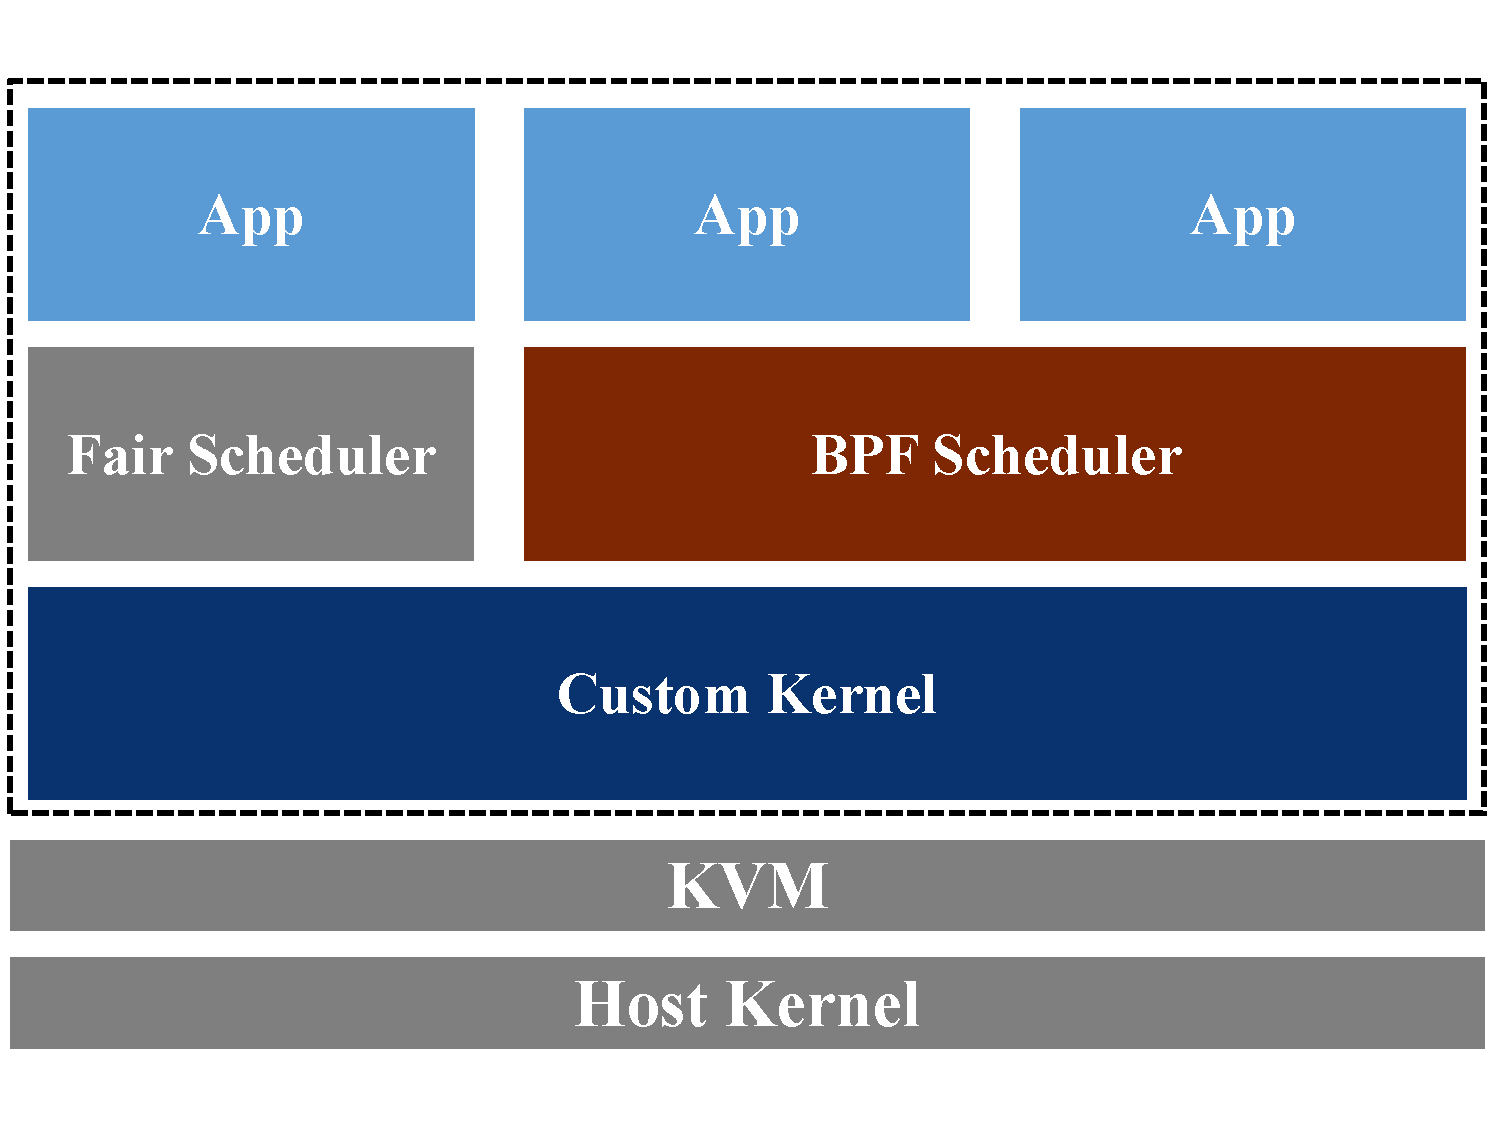
\includegraphics[width=\textwidth]{arch_dif_cz}
        \caption{Control Zone}
        \label{fig:arch_dif_cz}
    \end{subfigure}
    \hfill
    \begin{subfigure}[b]{0.45\textwidth}
        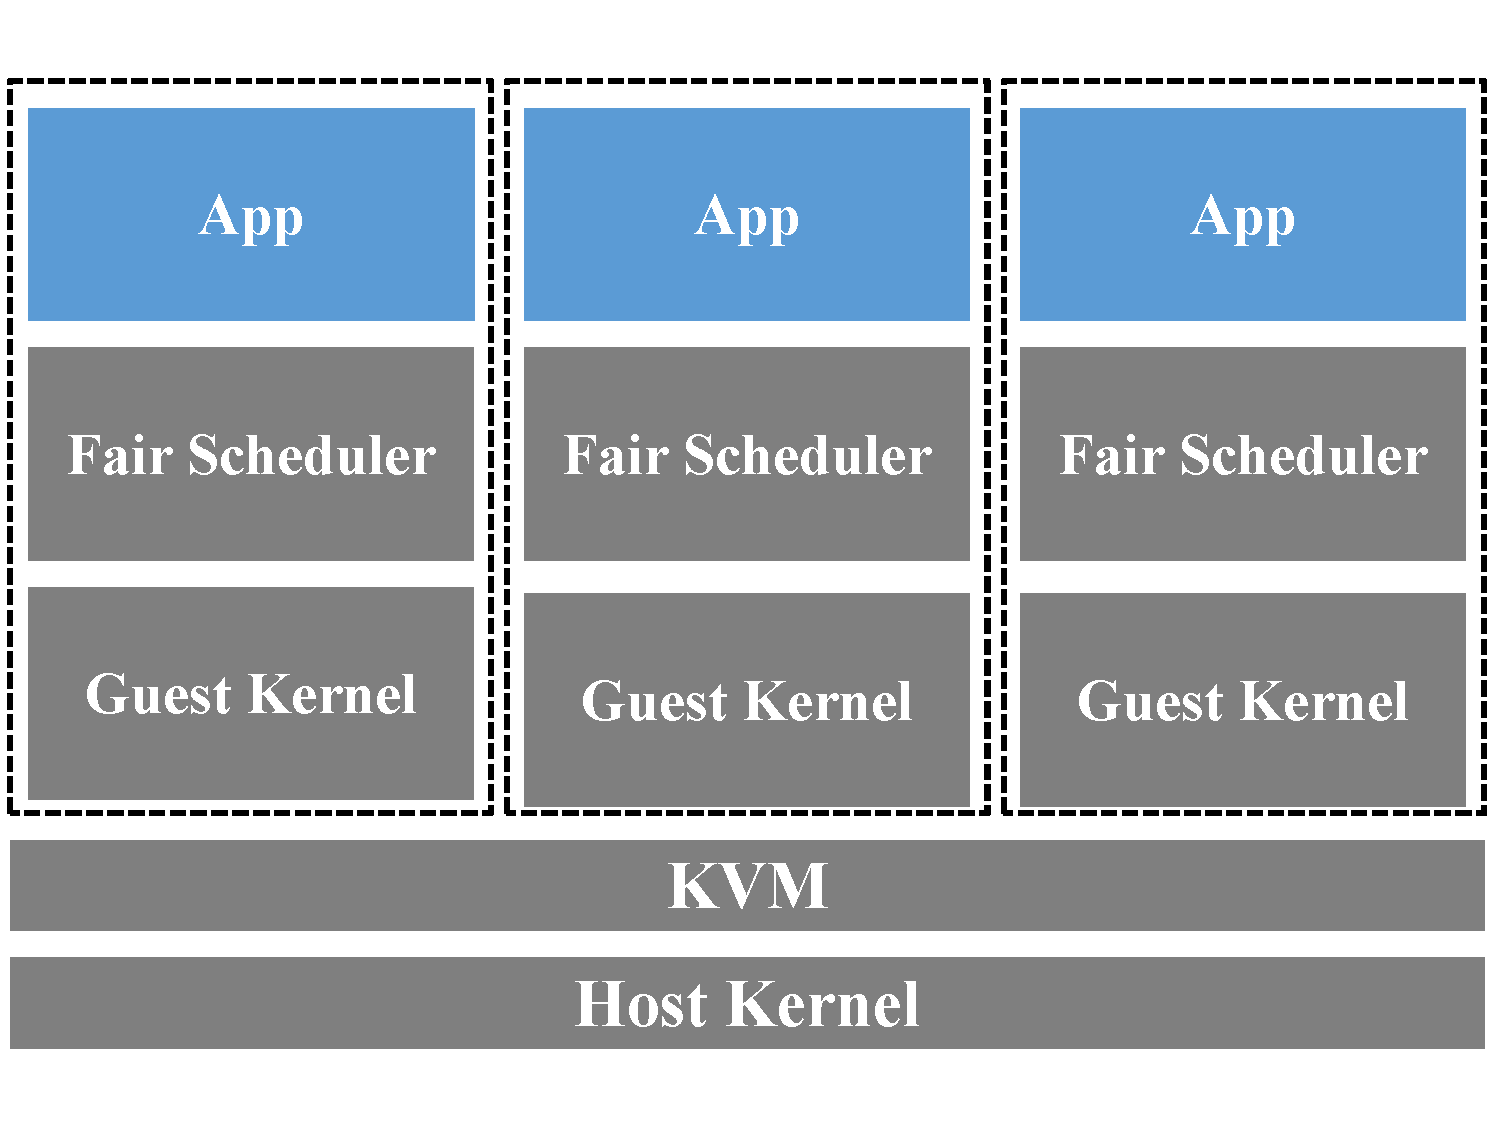
\includegraphics[width=\textwidth]{arch_dif_fc}
        \caption{Firecracker}
        \label{fig:arch_dif_fc}
    \end{subfigure}
\bicaption{\quad 沙箱结构差异}{\quad Sandbox Structure Differences}
\label{fig:arch_dif}
\end{figure}

\section{论文结构安排}

本文的主要内容分为六章,总体结构如图~\ref{fig:paper_organization}所示:

\begin{figure}[!htbp]
    \centering
    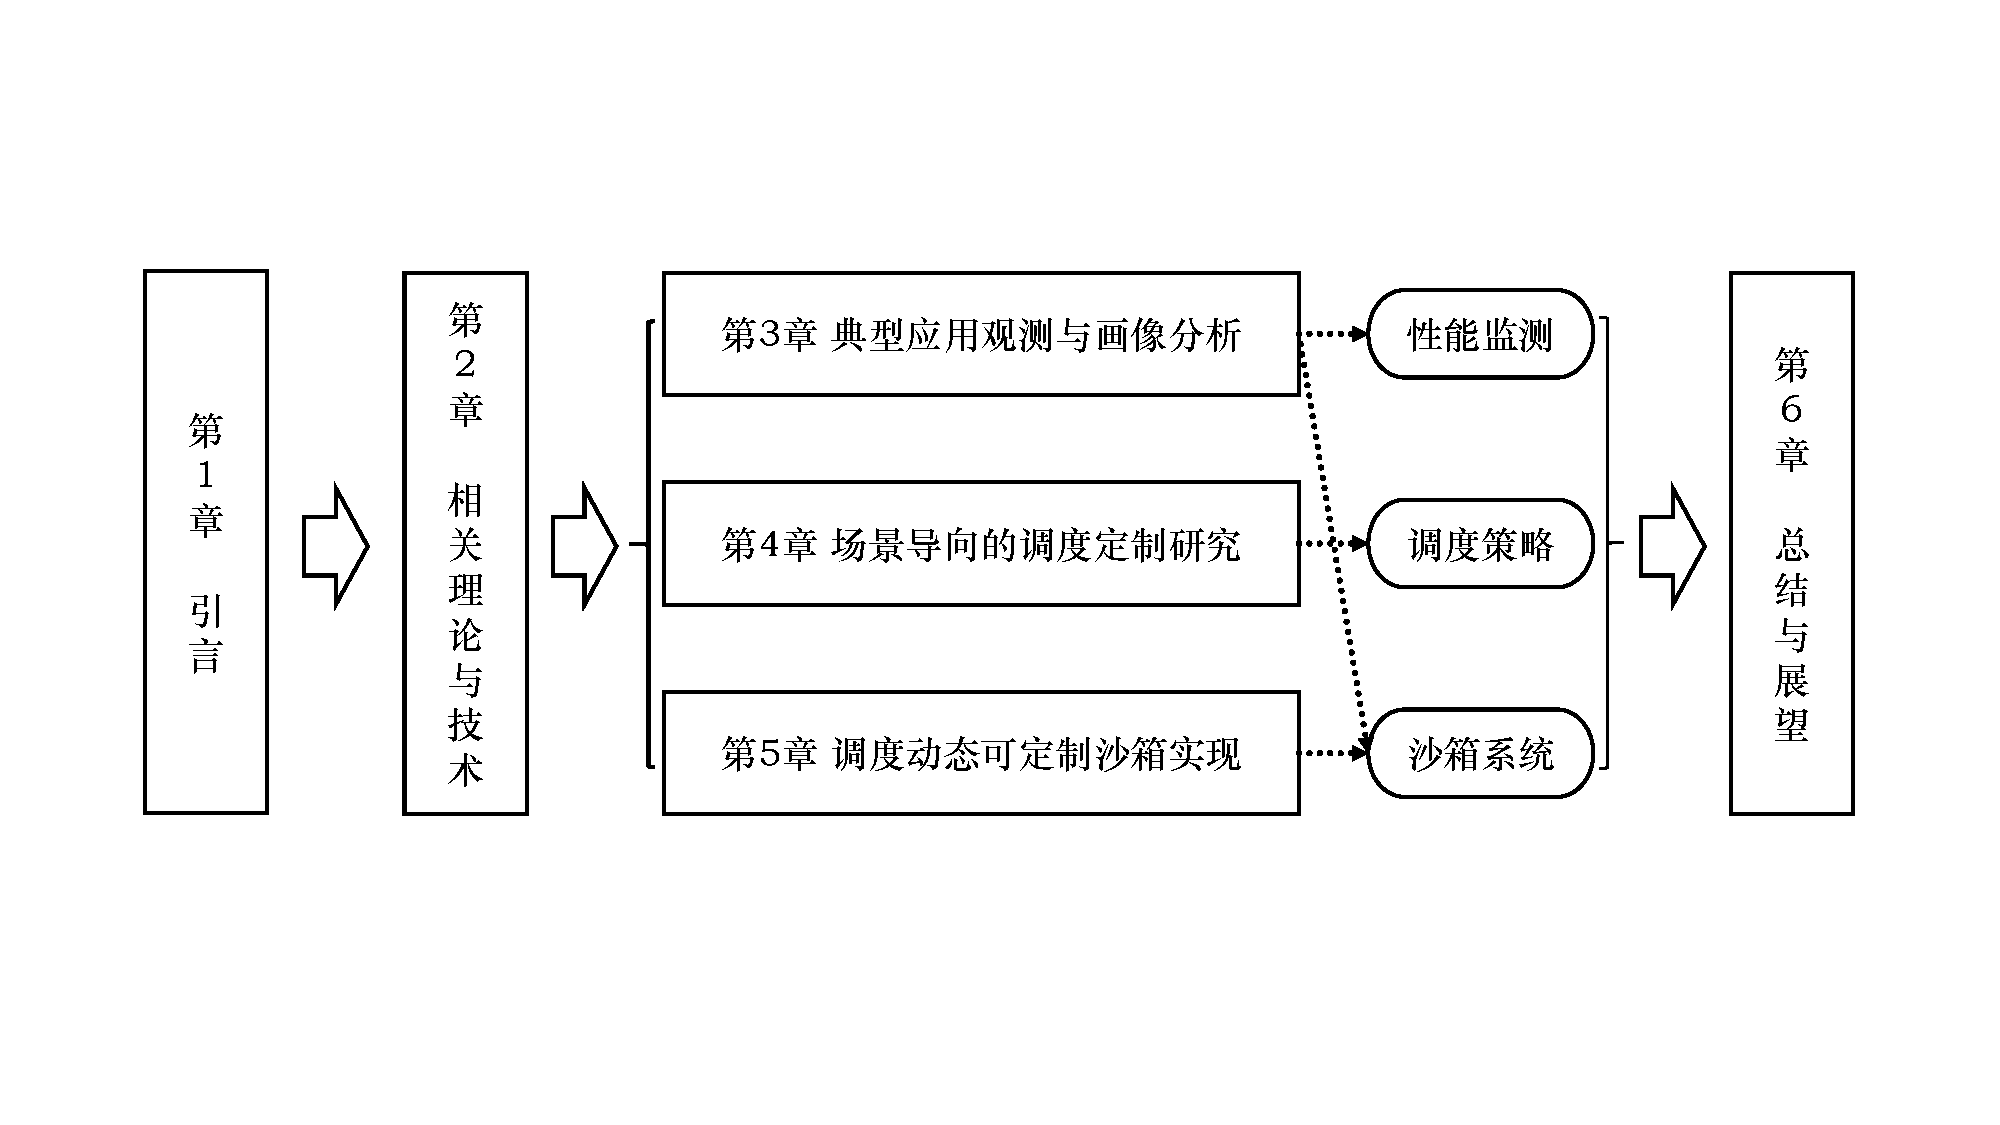
\includegraphics[width=1.0\textwidth]{paper_organization}
    \bicaption{\quad 本文组织架构}{\quad Paper Organization}
    \label{fig:paper_organization}
\end{figure}

第1章,相关背景说明,首先,阐述了本文的主要背景,并提出了本文要解决的面向混部场景的QoS保障问题。随后,从可观测性与劣化监测、围绕资源隔离的混部场景QoS保障、围绕任务调度的混部场景QoS保障三个方面分析了国内外研究现状。最后,阐述了本文的主要开展的工作,以及其对当前混部场景下QoS保障的贡献。

第2章,本文中所采用的技术说明,首先,分析了经典的Linux调度子系统的构成以及任务调度的决策过程,其次,介绍了本文中使用到的eBPF技术,阐述其核心特点,以及相较于内核模块等传统内核功能扩展技术的差异。随后,介绍了Sched Ext可扩展调度类,一种插件化内核调度器补丁集,说明了其实现的原理,为本文后续后续BPF Scheduler的实现进行铺垫,最后,介绍了沙箱技术以及相关的实现。

第3章,典型应用观测与画像分析,首先,介绍了云场景典型应用的选择方式及所挑选的应用,其次,针对虚拟机这一特殊场景,阐述了多维度指标采集可观测性系统的设计与实现,随后,分别对基准性能实验与干扰敏感度实验进行实验设计的阐述与最后的画像结果分析。

第4章,混部场景导向的任务调度机制定制,主要分为内核配置定制与Control Tower任务调度框架设计两个方面。在内核调度配置上,设计了响应度优先与吞吐量优先两种内核,而在Control Tower任务调度框架设计上,阐述了Control Tower的设计目标和实现原理,并扩展实现了CPU资源感知与网络资源感知两种Control Tower调度策略。

第5章,ControlZone的设计与实现。在第三、四章的基础之上,提供了一种内核可定制、调度运行时可变的沙箱系统,一方面能够针对不同的混部场景需要,在运行时层对Guest OS进行定制化,另一方面通过Control Tower任务调度框架提供插件化的调度器,从而能够在运行时根据应用的执行情况进行动态变化。

第6章,总结与展望。首先对于本文的工作进行了总结,分析各个工作的优势与不足,同时对未来在更多混部场景下进行调度定制进行了展望。